\documentclass[a4paper, 12pt]{article}

% Подключение русского языка.
\usepackage[russian]{babel}
\usepackage[utf8]{inputenc}
\usepackage[T2A]{fontenc}

% Настройка внешнего вида заголовков.
\usepackage{titlesec}
\newcommand{\chapterFont}{\fontsize{16}{15} \selectfont}
\newcommand{\chapterNumberFont}{\fontsize{14}{15} \selectfont}
\newcommand{\sectionFont}{\fontsize{14}{15} \selectfont}
\renewcommand\thesection{\thechapter.\arabic{section}.}
\titleformat{\chapter}[display]
{\normalfont \chapterFont \bfseries}{\centering \chapterNumberFont
	\chaptertitlename \ \thechapter}{10pt}{\centering \chapterFont}
\titlespacing{\chapter}{0pt}{8pt}{25pt}
\titleformat{\section}
{\normalfont \sectionFont \bfseries}{\centering \thesection}{6pt}
{\centering \sectionFont}
\titlespacing{\section}{0pt}{25pt}{5pt}
% Настройка размеров страниц.
\setlength{\parindent}{0pt} \renewcommand{\baselinestretch}{1.2} \topmargin = 0mm \textwidth =
175mm \textheight = 260mm \hoffset = -17.5mm \voffset = -25.5mm
% Подключение библиотек для изображений.
\usepackage{tcolorbox}
\usepackage{graphicx}
\usepackage{float}
% Подключение библиотек для математических символов.
\usepackage{amsthm}
\usepackage{parcolumns}
\usepackage{amsmath}
\usepackage{amsfonts}
% Настройка внешнего вида для теорем, утверждений и т.д.
\theoremstyle{definition}
\newtheorem*{theorem}{Теорема}
\newtheorem*{definition}{Определение}
\newtheorem*{example}{Пример}
\newtheorem*{remark}{Замечание}
\newtheorem*{solution}{Решение}

\begin{document}
\section*{Номер 52}
$$ \sqrt{y^2 + 1} dx = xy dy $$

\begin{solution}
    $$ \sqrt{y^2 + 1} dx = xy dy $$
    $$ \int \dfrac{dx}{x} = \int \dfrac{y dy}{\sqrt{y^2 + 1}} + C $$
    $$ \ln |x| = \sqrt{y^2 + 1} + C \text{ - общее решение} $$
    Проверим $x = 0$ и $\sqrt{y^2 + 1} = 0$ => $y^2 = -1$ => нет решения \par
    \textbf{Ответ: $x = 0$ - особая точка, $\ln |x| = \sqrt{y^2 + 1} + C$ общее решение.}

\end{solution}

\section*{Номер 54}

\begin{solution}
    $$ y' \ctg x + y = 2 $$
    $$ \dfrac{dy}{dx} \cdot \ctg x + (y - 2) = 0 | \cdot \dfrac{dx}{(y - 2) \cdot \ctg x}$$
    $$ \int \dfrac{d(y - 2)}{y - 2} + \int \dfrac{dx}{\ctg x} = 0 $$
    $$ \ln |y - 2| - \ln | \cos x | + C = 0 $$
    $$ \dfrac{|y - 2|}{|\cos x|} = C $$
    Доп условие: $y(x) \rightarrow -1$ при $x \rightarrow 0$, значит $\lim_{x \rightarrow 0} y(x) = 1$
    $$ -1 = C_1 \cdot \cos 0 + 2 \Rightarrow -1 = C_1 + 2 \Rightarrow C_1 = -3 $$
    $$ y = 2 - 3 \cos x $$
    \textbf{Ответ: $y = 2 + C_1 \cdot \cos x$ - общее решение, с учетом усл: $y = 2 - 3 \cdot \cos x$.}
\end{solution} \pagebreak

\section*{Номер 67} 

\begin{solution}
    $$ 3y^2 y' + 16x = 2xy^3 $$  
    $$ 3y^2 \dfrac{dy}{dx} + 16x - 2xy^3 = 0 $$  
    $$ 3y^2 dy + (16x - 2xy^3) dx = 0 $$  
    Разделим на $(8 - y^3)$:  
    $$ \dfrac{3y^2 dy}{y^3 - 8} = \dfrac{2x dx}{1} $$  

    Введём замену:  
    $$ t = y^3 - 8, \quad dt = 3y^2 dy $$  
    Тогда уравнение принимает вид:  
    $$ \int \dfrac{dt}{t} = \int 2x dx + C $$  
    $$ \ln |y^3 - 8| = x^2 + C $$  
    $$ e^{\ln |y^3 - 8|} = e^{x^2 + C} $$  
    $$ y^3 - 8 = e^{x^2} e^C $$  

    Обозначим $C_1 = e^C$:  
    $$ y^3 - 8 = C_1 e^{x^2} $$  
    $$ y = \sqrt[3]{C_1 e^{x^2} + 8} $$  

    Найдём частное решение.  
    По условию, $y(x)$ ограничена при $x \to +\infty$, значит $C_1 = 0$.  
    Тогда  
    $$ y = \sqrt[3]{8} = 2 $$  

    \textbf{Ответ:} общее решение:  
    $$ y = \sqrt[3]{C_1 e^{x^2} + 8} $$  
    c учетом условия:  
    $$ y = 2. $$
\end{solution}


\pagebreak
\section*{Номер 102}

$$ (x - y) dx + (x + y) dy = 0 $$

\begin{solution}
    1) Проверерим на однородность: $x, y \rightarrow kx, ky$ \par
    $$ (kx - ky) dx + (kx + ky) dy = 0 $$
    $$ k[(x - y) dx + (x + y) dy] = 0 $$

    2) Замена $z = \dfrac{y}{x} \Rightarrow y = zx \Rightarrow dy = zdx + xdz$ \par
    $$ (x - zx) dx + (x + zx) \cdot (zdx + xdz) = 0 $$
    $$ xdx - zxdx + xzdx + x^2 dz + z^2 xdx + x^2 zdz = 0 $$

    $$ (x + x^2 z) dx + (x^2 + x^2 z) dz = 0 $$  
    Преобразуем:  
    $$ x(1 + z^2) dx + x^2(1 + z^2) dz = 0 $$  
    Разделяем переменные:  
    $$ \int \frac{dx}{x} = - \int \frac{1 + \frac{z}{1 + z^2} dz}{1 + z^2} $$  
    
    Распишем правую часть:  
    $$ \int \frac{dx}{x} = - \int \frac{z}{1 + z^2} dz - \int \frac{1}{1 + z^2} dz $$  
    Решение интегралов:  
    $$ \int \frac{z}{1 + z^2} dz = \frac{1}{2} \ln(1 + z^2), \quad \int \frac{dz}{1 + z^2} = \arctg z $$  
    Получаем:  
    $$ C + \ln |x| = -\arctg z - \frac{1}{2} \ln(1 + z^2) $$  
    Возводим в экспоненту:  
    $$ e^{C + \ln |x|} = e^{-\arctg z - \frac{1}{2} \ln(1 + z^2)} $$  
    $$ C + \ln |x| = -\arctg \frac{y}{x} - \frac{1}{2} \ln \left( 1 + \frac{y^2}{x^2} \right) $$  
    $$ C - 2 \ln |x| = 2 \arctg \frac{y}{x} + \ln \left( \frac{x^2 + y^2}{x^2} \right) $$  
    $$ \ln (x^2 + y^2) - \ln x^2 = \ln (x^2 + y^2) - 2 \ln x $$  
    $$ 2 \arctg \frac{y}{x} + \ln (x^2 + y^2) = C + 2 \ln |x| - 2 \ln x $$  
    \textbf{Итоговое общее решение: } 
    $$ \ln (x^2 + y^2) = C - \arctg \frac{y}{x} $$  
    
    Проверяем условия:  
    $$ x^2 = 0, \quad 1 + z^2 = 0 $$  
    Поскольку решений нет, записываем:  
    $$ \text{Нет решений.} $$
\end{solution}

\section*{Задача 114}
$$ (2x + y + 1)dx - (4x + 2y - 3) dy = 0 $$

\begin{solution}
    Проверяем однородность:  
    $$ 2xy + 4x + y + 1 = 0 $$  
    $$ y = -2x - 1 $$  
    $$ 4x + 2y + 3 = 0 $$  
    Подставляя $y = -2x - 1$:  
    $$ 4x + 2(-2x - 1) + 3 = 0 $$  
    $$ 4x - 4x - 2 + 3 = 0 $$  
    $$ 1 \neq 0, \quad \text{нет решений.} $$  

    \textbf{Прямые не пересекаются.}  

    Рассмотрим уравнение:  
    $$ \frac{dy}{dx} = \frac{2x + y + 1}{4x + 2y - 3} $$  
    Введём замену:  
    $$ z = 2x + y, \quad dz = 2dx + dy $$  
    Тогда:  
    $$ dz - 2dx = \frac{2x + y + 1}{4x + 2y - 3} dx $$  
    $$ \frac{dz}{dx} = \frac{2x + y + 1}{4x + 2y - 3} + 2 $$  
    Выразим через $z$:  
    $$ z' = \frac{z + 1}{2z - 3} $$  

    Решаем методом разделяющихся переменных:  
    $$ \frac{dz}{dx} = \frac{5(z - 1)}{2z - 3} $$  
    $$ \int \frac{2z - 3}{z - 1} dz = \int 5dx $$  
    Разбиваем дробь:  
    $$ \int 2 \frac{z - 1}{z - 1} dz - \int \frac{dz}{z - 1} = \int 5 dx $$  
    $$ \int 2 dz - \int \frac{dz}{z - 1} = \int 5 dx $$  
    $$ 2z - \ln |z - 1| = 5x + C $$  
    Возвращаемся к $z$:  
    $$ 2(2x + y) - \ln |2x + y - 1| = 5x + C $$  
    $$ 4x + 2y - \ln |2x + y - 1| = 5x + C $$  
    $$ 2x + y - 1 = e^{\frac{C - 5x}{2}} $$  

    Общее решение:  
    $$ 2x + y + 1 = C_3 e^{2y - x} $$  
\end{solution}\pagebreak

\section*{Номер 121}

$$ x^3 \left( y' - x \right) = y^2 $$

\begin{solution}
    Проверим на однородность:  
    $$ x^3 \frac{dy}{dx} = y^2 $$  
    Неоднородное, так как при $x, y \to kx, ky$ не было бы явного $x$.  

    1) Замена:  
    $$ y = z x^m $$  

    Подставляем:  
    $$ x^3 \left( m z x^{m-1} + x^m z' - x \right) = z^2 x^{2m} $$  
    Уравнение будет однородным, если:  
    $$ 2m = 3 + m + 1 \Rightarrow m = 2 $$  

    2) Подставим $m = 2$:  
    $$ x^3 \left( 2z x + x^2 z' - x \right) = z^2 x^4 $$  

    Теперь уравнение однородное.  

    3) Введём замену:  
    $$ t = x, \quad z = \frac{y}{x^2} $$  
    Тогда:  
    $$ dz = \frac{dy}{x^2} - \frac{2y dx}{x^3} $$  
    Подставляем:  
    $$ dz = \frac{dx}{x} + x z' $$  

    Преобразуем уравнение:  
    $$ z' = -t + x L' $$  

    Решаем методом разделяющихся переменных:  
    $$ 2t + 2t x' - t^4 = 0 $$  
    $$ 2t dx + 2t x^2 dx - t^4 dx = 0 $$  
    $$ 2t dt = (t^4 - 2t) dx $$  
    $$ 2t dt = (t^2 - 1) dx $$  

    Итоговое уравнение с разделяющимися переменными:  
    $$ \int \frac{2t dt}{(t^2 - 1)} = \int dx $$  

    Решение в общем виде:  
    $$ (x^2 - y) \ln C x = x^2 \text{ - общее решение.} $$  
\end{solution}

\pagebreak
\section*{Номер 140}

$$ x^2 y' + xy + 1 = 0 $$

\begin{solution}
    Решим однородное: $x^2y' + xy = 0$

    $$ \frac{dy}{dx} + \frac{y}{x} = 0 $$  
    $$ \int \frac{dy}{y} = -\int \frac{dx}{x} $$  

    Интегрируем:  
    $$ \ln |y| = -\ln |x| + C $$  
    $$ \ln |y| + \ln |x| = C $$  
    $$ \ln |yx| = C $$  
    $$ yx = e^C $$  
    Обозначим $e^C = C_1$:  
    $$ yx = C_1 $$  
    $$ y = \frac{C_1}{x} $$  

    Подставляем в неоднородное уравнение:  
    $$ x^2 \left( \frac{C(x) \cdot x - x}{x^2} \right) + x \cdot \frac{C(x)}{x} + 1 = 0 $$  

    Упрощаем:  
    $$ C(x) \cdot x - x + C(x) + x + 1 = 0 $$  
    $$ C(x) \cdot x + C(x) + 1 = 0 $$  

    Найдём $C(x)$:  
    $$ \frac{dC}{dx} \cdot x = -1 $$  
    $$ \int dC = \int \frac{dx}{x} $$  

    Интегрируем:  
    $$ C(x) = -\ln |x| + C_1 $$  
    $$ y = -\ln |x| + C_1 $$  

    Общее решение:  
    $$ xy = C - \ln |x| $$  
    Особых решений нет.  
\end{solution}\pagebreak

\section*{Номер 149}

$$ y' = \dfrac{y}{3x - y^2} $$

\begin{solution}
    $$ y = y' \cdot (3x - y^2) $$

    $$ \frac{dx}{dy} = \frac{y}{3x - y^2} $$  
    Уравнение имеет вид линейного относительно $x$:  
    $$ x' + P(y)x = Q(y) $$  

    Решим как однородное:  
    $$ x = y^z $$  
    $$ \frac{dx}{dy} = 3 \frac{x}{y} $$  

    Интегрируем:  
    $$ \int \frac{dx}{3x} = \int \frac{dy}{y} $$  
    $$ \frac{1}{3} \ln |x| = \ln |y| + C $$  
    $$ e^{\frac{1}{3} \ln |x|} = e^{\ln |y| + C} $$  
    $$ |x| = y^3 e^C $$  

    Обозначим $C_1 = e^C$:  
    $$ x = y^3 C_1 $$  

    Теперь найдём $C(y)$:  
    $$ 3y^2 C(x) + y^3 C'(x) = 3 \cdot y^4 C(x) - y $$  
    Разделим на $y^3$:  
    $$ C'(x) = -y $$  
    Интегрируем:  
    $$ C(x) = -\frac{1}{4} y^4 + C_1 $$  
    $$ x = y^3 \left( -\frac{1}{4} y^4 + C_1 \right) $$  
    $$ x = y^2 - \frac{1}{4} y^5 + C y^3 $$  

    \textbf{Общее решение:}  
    $$ x = y^2 + y^3 C $$  
    Особых решений нет.  
\end{solution}\pagebreak

\section*{Номер 155}

$$ xy dy = (y^2 + x) dx $$

\begin{solution}
    $$ \dfrac{dy}{dx} = \dfrac{y^2 + x}{xy} \Rightarrow y' = \dfrac{y^2 + x}{xy} $$
    $$ x \cdot y' = y + x \cdot y^{-1}, n = -1 \leftarrow \text{уравнение Бернулли} $$
    Замена $z = \dfrac{1}{y^{n - 1}} \Rightarrow z = \dfrac{1}{y^{-2}} = y^2 \Rightarrow y = \sqrt{z}$, $ dz = 2y dy \Rightarrow dy = \dfrac{dz}{2 \sqrt{z}}$ \par
    $$ x \cdot \dfrac{dy}{dx} = y + \dfrac{x}{y} \rightarrow \dfrac{x}{dx} \cdot \dfrac{dz}{2 \sqrt{z}} = \sqrt{z} + \dfrac{x}{\sqrt{z}} $$
    $$ x \cdot z' = 2z + 2x $$
    Замена $t = \dfrac{z}{x} \Rightarrow z = tx \Rightarrow z' = t + xt'$ \par
    $$ \int \dfrac{dt}{t + 2} = \int \dfrac{dx}{x} $$
    $$ \ln |t + 2| = \ln |x| + C $$
    $$ |t + 2| = |x| \cdot e^C $$
    Обратная замена $\dfrac{z}{x} + z = C x \rightarrow y^2 = Cx^2 - 2x$ - общее решение. 

\end{solution}\pagebreak
\section*{Номер 252}

$$ xy' (xy' + y) = 2y^2 $$

\begin{solution}
    $$ D = x^2 y^2 - 4(-2y^2) \cdot x = x^2 y^2 + 8xy^2 = (3xy)^2 $$
    $$ y_{1,2}' = \frac{-xy \pm 3xy}{2x^2} \Rightarrow y_1' = -\dfrac{2y}{x}, \quad y_2' = \dfrac{y}{x} $$

    1) $$ y' = -\frac{2y}{x} $$
    $$ \frac{dy}{dx} = -\frac{2y}{x} $$
    $$ \int \frac{dy}{y} = \int -\frac{2dx}{x} $$
    $$ \ln |y| = -2 \ln |x| + \ln C $$
    $$ y = C x^{-2} $$
    $$ yx^2 = C $$

    2) $$ y' = \frac{y}{x} $$
    $$ \frac{dy}{dx} = \frac{y}{x} $$
    $$ \int \frac{dy}{y} = \int \frac{dx}{x} $$
    $$ \ln |y| = \ln |x| + \ln C $$
    $$ y = Cx $$
\end{solution}\pagebreak

\section*{Номер 268}

$$ x ((y')^2 - 1) = 2y' $$

\begin{solution}
    $$ x(y')^2 - 2y' - x = 0 \text{ - метод введения параметра.}$$
    $$ y' = p => \dfrac{dy}{dx} = p \Rightarrow dy = p \cdot dx \Rightarrow dx = \dfrac{dy}{p} $$
    $$ x(p^2 - 1) = 2p $$
    $$ x = \dfrac{2p}{p^2 - 1} $$
    $$ \dfrac{dy}{p} = -2 \dfrac{(p^2 + 1)}{(p^2 - 1)^2} dp $$
    $$ dy = \dfrac{-2p \cdot (p^2 + 1)}{(p^2 - 1)}dp $$
    $$ y = -2 \int p \left( \frac{p^2 - 1}{(p^2 - 1)^2} + \frac{2p}{(p^2 - 1)^2} \right) dp $$
    $$ = -2 \int \frac{p}{p^2 - 1} dp - 2 \int \frac{2p^2}{(p^2 - 1)^2} dp $$
    $$ = - \int \frac{d (p^2 - 1)}{p^2 - 1} - 2 \int \frac{d (p^2 - 1)}{(p^2 - 1)^2} $$
    $$ \Rightarrow y = -\ln |p^2 - 1| + \frac{2}{p^2 - 1} + C $$

    $$ x = \frac{2p}{p^2 - 1} $$

    Решение общее, особых нет.

    \textbf{Найдём особое решение:}

    Дифференцируем обе части исходного уравнения по $y'$:
    $$ 2xy' = 2 \Rightarrow y'' = \frac{X}{x} $$
    Подставляем в исходное уравнение:
    $$ x \left( \frac{1}{X^2} \right)^2 - 1 = \frac{2}{x} \Rightarrow 2 \cdot \frac{1}{X^2} = 1 \Rightarrow \frac{1}{X^2} = \frac{1}{2} $$
    $$ x^2 - 1 \text{ (невозможно)} \Rightarrow \text{особых решений нет} $$
\end{solution}\pagebreak

\section*{Номер 270}
$$ y' \cdot (x - \ln y') = 1 $$

\begin{solution}
    $$ y' \cdot x x - y' \cdot \ln y' = 1 $$
    $$ x = \ln y' + \dfrac{1}{y'} $$
    Вести параметр $\dfrac{dy}{dx} = p$
    $$  = \ln p + \dfrac{1}{p} $$
    $$ y = \int \left( \frac{1}{p} - \frac{1}{p^2} \right) dp $$
    $$ = \int 1 - \frac{1}{p} dp $$
    $$ = p - \ln p + C $$
    
    $$ x = \ln p + \frac{1}{p} $$
    
    \text{Общее решение, особых решений нет.}
    
    \textbf{Найдём особое решение:}
    
    Дифференцируем уравнение по $y'$:
    $$ x - \ln y' - 1 = 1 $$
    $$ y' = e^{x - 2} $$
    
    Подставляем в исходное уравнение:
    $$ e^{x - 2} \cdot (x - \ln e^{x - 2}) = 1 $$
    $$ e^{x - 2} \cdot (x - x + 2) = 1 $$
    $$ e^{x - 2} = \frac{1}{2} $$
    
    Такого решения нет, следовательно, особых решений нет.
\end{solution}
\pagebreak
\section*{Номер 212}

$$ (2x^2y^3 - 1)y dx + (4x^2y^3 - 1)x dy = 0 $$

\begin{solution}
    1) $$ (2x^2y^4 - y)_y' = (4x^3y^3 - x)_x' $$
    $$ 8x^2y^3 - 1 = 12x^2y^3 - 1 \text{ - неверно. Проверка в полных диф-ах не пройдена.} $$
    2) $$ 2x^2y^4dx - ydx + 4x^3y^3dy - xdy = 0 $$
    $$ 2x^2y^2 \cdot d(xy^2) - d(xy) = 0 $$
    Замена $$ \begin{cases}
        z = xy \Rightarrow z^2 = x^2y^2 \\
        t = xy^2
    \end{cases} $$

    $$ 2z^2 dt - dz = 0 $$
    $$ 2 \int dt - \int \dfrac{dz}{z^2} = 0 $$
    $$ 2xy^2 + \dfrac{1}{xy} = C \text{ - общее решение, а $x = 0, y = 0$ - особые точки.}$$
\end{solution}

\section*{Номер 257}
$$ (y')^2 - 2xy' = 8x^2 $$
\begin{solution}
    $$ D = 4x^2 = 36x^2 $$
    $$ y_{1,2}' = \dfrac{2x \pm 6x}{2} $$
    Общие решения: $ y_1 = 2x^2 + C \quad y_2 = -x^2 + C $
    
\end{solution}

\section*{Номер 274}

$$ y = (y' - 1) \cdot e^{y'}$$

\begin{solution}
    $$ p = y' \Rightarrow \dfrac{dy}{dx} = p \Rightarrow dx = \dfrac{dy}{p} $$
    $$ y = (p - 1) \cdot e^p $$
    $$ dx = \dfrac{dy}{p} = e^p dp $$
    $$ x = e^p + C \quad y = (p - 1) \cdot e^p \quad y = -1 $$
\end{solution}
\pagebreak
\section*{Номер 307}

$$ y^3 - y' e^{2x} = 0 $$

\begin{solution}
    Введём замену:
    $$ y' = p \Rightarrow dy = p dx \Rightarrow dx = \frac{dy}{p} \Rightarrow dy = p dx $$

    Подставим в уравнение:
    $$ p^3 - p e^{2x} = 0 $$

    Разделим на $p$ (если $p \neq 0$):
    $$ p^2 - e^{2x} = 0 $$

    Найдём корни:
    $$ p_{1,2} = \pm e^x $$

    Тогда:
    $$ y'_{1,2} = \pm e^x \Rightarrow \frac{dy}{dx} = \pm e^x $$

    Интегрируем:
    $$ \int dy = \int \pm e^x dx $$

    $$ y = C \pm e^x $$
\end{solution}

\section*{Номер 309}

$$ (1 - x^2) dy + xy dx = 0 $$

\begin{solution}
    Разделим уравнение на $(1 - x^2) y$:
    $$ \frac{1}{y} dy = \frac{x dx}{1 - x^2} $$

    Интегрируем:
    $$ \int \frac{dy}{y} = \int \frac{x dx}{1 - x^2} $$

    Решаем:
    $$ \ln |y| = \frac{1}{2} \ln |1 - x^2| + \ln |C| $$

    $$ 2 \ln |y| = \ln |1 - x^2| + \ln |C| $$

    $$ y^2 = C (1 - x^2) $$

    Это общее решение. 

    Особые решения при $ x = \pm 1 $.
\end{solution} \pagebreak

\section*{Номер 310}

$$ y'' + 2(x - 1)y' - 2y = 0 $$

\begin{solution}
    Разделим уравнение на 2:
    $$ \frac{y''}{2} + (x - 1)y' - y = 0 $$
    Перепишем в стандартном виде:
    $$ y'' = y - (x - 1)y' $$
    Это уравнение Клеро.

    Общее решение имеет вид:
    $$ y(x, C) = \frac{C^2}{2} + (x - 1)C $$

    Введём замену:
    $$ p = y', \quad dy = p dx $$
    Тогда:
    $$ y = \frac{p^2}{2} + (x - 1)p $$

    Дифференцируем:
    $$ dy = p dp + (x - 1) dp + p dx $$
    Преобразуем:
    $$ (p + x - 1) dp = 0 $$

    Отсюда:
    $$ \int dp = 0, \quad p + x - 1 = 0 $$

    Следовательно:
    $$ p = C, \quad p = -x + 1 $$

    Тогда:
    $$ y(x) = \frac{(1 - x)^2}{2} + (x - 1)(1 - x) $$

    Итоговый результат:
    $$ y(x) = -\frac{(1 - x)^2}{2} $$
\end{solution}\pagebreak

\pagebreak

\section*{Задача 1104}
Найти общее решение дифференциального уравнения:
$$(1 - x)y'' - 2y' + y = 0$$

\begin{solution}
   Решим задачу методом рядов.

   1) Предположим, что решение имеет вид:
   $$y = \sum_{k = 0}^{\infty} y_k x^k$$

   2) Тогда:
   $$y' = \sum_{k = 0}^{\infty} y_k k x^{k-1}$$
   $$y'' = \sum_{k = 0}^{\infty} y_k k(k-1) x^{k-2}$$

   3) Подставляем в исходное уравнение:
   $$\sum_{k = 0}^{\infty} y_k k(k-1)x^{k-2} - y_k k(k-1)x^{k-1} - 2y_k kx^{k-1} + y_k x^k = 0$$

   4) Приравнивая коэффициенты при $x^k$:
   $$y_k - k(k+1)y_{k+1} - 2(k+1)y_{k+1} + y_{k+2}(k+1)(k+2) = 0$$

   5) Рекуррентное соотношение:
   $$y_{k+2} = \frac{y_{k+1}(k+1)(k+2) - y_k}{(k+1)(k+2)}$$

   6) Два линейно независимых решения:

   Первое решение ($y_0 = 1, y_1 = 0$):
   $$y_1 = 1 - \frac{1}{2}x - \frac{1}{2}x^2 - \frac{11}{24}x^3 + \cdots$$

   Второе решение ($y_0 = 0, y_1 = 1$):
   $$y_2 = x + \frac{5}{6}x^2 + \frac{3}{4}x^3 + \cdots$$

   Таким образом, общее решение:
   $$y = c_1y_1 + c_2y_2$$
   где $c_1$ и $c_2$ — произвольные константы.
\end{solution}
\section*{Задача 1106}
Найти общее решение дифференциального уравнения:
$$y'' - xy' + xy = 0$$

\begin{solution}
1) Предположим решение в виде степенного ряда:
   $$y = \sum_{k = 0}^{\infty} y_k x^k$$

2) Производные:
   $$y' = \sum_{k = 0}^{\infty} y_k k x^{k-1}$$
   $$y'' = \sum_{k = 0}^{\infty} y_k k(k-1) x^{k-2}$$

3) Подставляем и приравниваем коэффициенты:
   $$y_{k+3} = \frac{y_{k+1}(k+1) - y_k}{(k+3)(k+2)}$$

4) Три линейно независимых решения:

   Первое решение ($y_0 = 1, y_1 = 0, y_2 = 0$):
   $$y_1 = 1 - \frac{1}{6}x^3 - \frac{1}{40}x^5 + \cdots$$

   Второе решение ($y_0 = 0, y_1 = 1, y_2 = 0$):
   $$y_2 = x + \frac{1}{6}x^3 - \frac{1}{12}x^4 + \frac{1}{40}x^5 + \cdots$$

   Третье решение ($y_0 = 0, y_1 = 0, y_2 = 1$):
   $$y_3 = x^2 + \frac{1}{6}x^4 - \frac{1}{40}x^5 + \cdots$$

Таким образом, общее решение:
$$y = c_1y_1 + c_2y_2 + c_3y_3$$
где $c_1$, $c_2$ и $c_3$ — произвольные константы.
\end{solution}

\section*{Задача 1110}
Найти общее решение дифференциального уравнения:
$$ xy'' + 2y' + xy = 0 $$
\begin{solution}
    1) При $x_0 = 0 $ : $ p_0(0) = 0 $ => $ \sum_{k = 0}^{\infty} y_k x^{k + \alpha} $ \par
    2) Преобразуем: $$ \sum_{k = 0}^{\infty} y_k (k + \alpha) (k + \alpha - 1) x^{k + \alpha - 2 + 1} + 2 \sum_{k = 0}^{\infty} y_k (k + \alpha) x^{k + \alpha - 1} + \sum_{k = 0}^{\infty} y_k x^{k + \alpha + 1} = 0 $$
    3) min степень $x$: $ k + \alpha - 1 $, $ k = 0 $ => $ \alpha - 1 $ => \par
    при $ k = 0 $: $ y_0 \alpha (\alpha - 1) x^{\alpha - 1} + 2 y_0 \alpha x^{\alpha - 1} + y_0 x^{\alpha + 1} $ \par
    $ y_0 (\alpha (\alpha - 1) + 2 \alpha) $, где $ (\alpha (\alpha - 1) + 2 \alpha) = 0 $, при $ x^{\alpha - 1} $ (минимальная степень $x$) \par
    $ \alpha (\alpha + 1) = 0 $ => $ \alpha = 0 $; $-1$, но берем $-1$, т.к. $\alpha = 0$ делает ряд обычным. \par
    4) Получаем ряд: $$ \sum_{k = 0}^{\infty} \underset{k = p + 2}{y_k (k - 1) (k - 2) x^{k - 2}} + 2 \sum_{k = 0}^{\infty} \underset{k = p + 2}{y_k (k - 1) x^{k - 2}} + \sum_{k = 0}^{\infty} \underset{k = p}{y_k x^k = 0} $$
    5) При $ x^p $ : $$ y_{p + 2} (p + 1) + 2y_{p + 2} (p + 1) + y_p = 0 $$
    $$ y_{p + 2} (p + 1) (p + 2) + y_p = 0 $$
    $$ y_{p + 2} = -\dfrac{y_p}{(p + 1) (p + 2)} $$
    6) Построим матрицу: 
    $
        \begin{array}{ccc}
                  & 1) & 2) \\
            y_0 = & 1  & 0  \\
            y_1 = & 0  & 1  \\
        \end{array}
    $ \par
    \quad1) $ y_2 = -\dfrac{1}{2} = -\dfrac{1}{2!} $, $ y_3 = 0 $, $ y_4 = -\dfrac{-\dfrac{1}{2}}{3 \cdot 4} = \dfrac{1}{24} = \dfrac{1}{4!} $, $\cdots$ => \par
    => $ y_1 = \dfrac{1}{x} - \dfrac{x}{2!} + \dfrac{x^3}{4!} - \dfrac{x^5}{6!} + \cdots $\par
    \quad2) $ y_2 = 0 $, $ y_3 = -\dfrac{1}{1 \cdot 2 \cdot 3} = -\dfrac{1}{3!} $, $ y_4 = 0 $, $\cdots$ => \par
    => $ y_2 = 1 - \dfrac{x^2}{3!} + \dfrac{x^4}{5!} - \dfrac{x^6}{7!} + \cdots $ \par
    7) Общее решение будет выглядить так: $ y = c_1y_1 + c_2y_2 $
\end{solution}\pagebreak

\pagebreak\section*{Задача 1109}
Найти общее решение дифференциального уравнения: $$ y''' - xy'' + (x - 2)y' + y = 0 $$
\begin{solution}
    1) При $x_0 = 0 $, $ p_0(0) \neq 0 $ => $ y = \sum_{k = 0}^{\inf} y_k x^k $. \par
    2) Преобразуем: $$ \sum_{k = 0}^{\inf} \underset{k = p + 3}{k (k - 1) (k - 2) y_k x^{k - 3}} - \sum_{k = 0}^{\inf} \underset{k = p + 1}{k (k - 1) y_k x^{k -2 + 1}} + \sum_{k = 0}^{\inf} \underset{k = p}{k y_k x^{k - 1 + 1}} - 2 \sum_{k = 0}^{\inf} \underset{k = p + 1}{k y_k x^{k - 1}} + \sum_{k = 0}^{\inf} \underset{k = p}{y_k x^k} = 0 $$
    При $ x^p $ : $$ (p + 3) (p + 2) (p + 1) y_{p + 3} - (p + 1) p y_{p + 1} + p y_p - 2 (p + 1) + y_p = 0 $$
    Сократим $ (p + 1) $ : $$ (p + 3) (p + 2) y_{p + 3} - (p + 2) y_{p + 1} + y_p = 0 $$
    3) Выразим $ y $ : $$ y_{p + 3} = \frac{y_{p + 1}}{p + 3} - \frac{y_p}{(p + 3)(p + 2)} $$
    4) Построим единичную матрицу: \par
    $$\begin{array}{c ccc}
                      & 1) & 2) & 3) \\
                y_0 = & 1  & 0  & 0  \\
                y_1 = & 0  & 1  & 0  \\
                y_2 = & 0  & 0  & 1  \\
            \end{array}$$\par
    \quad1) $ y_3 = 0 - \frac{1}{6} = -\frac{1}{6} $, $ y_4 = 0 $, $ y_1 = 1 - \frac{x^3}{6} + 0 + \cdots $\par
    \quad2) $ y_3 = \frac{1}{3} - 0 = \frac{1}{3} $, $ y_4 = -\frac{1}{12} $, $ y_2 = x + \frac{x^3}{3} - \frac{x^4}{12} + \cdots $\par
    \quad3) $ y_3 = 0 $, $ y_4 = \frac{1}{4} $, $ y_3 = x^2 + \frac{x^4}{4} + \cdots $\par
    5) Таким образом общее решение: $$ y = c_1y_1 + c_2y_2 + c_3y_3 $$ где $c_1$, $c_2$ и $c_3$ - произвольные константы.

\end{solution}\pagebreak
\pagebreak\section*{Задача 1114}
Найти общее решение дифференциального уравнения: $$ x^2y'' + 2xy' - (x^2 + 2x + 2)y = 0. $$
\begin{solution}
    1) При $ x_0 = 0, p_0(0) = 0 $ => Общий случай $ y = \sum_{k = 0}^{+\infty} y_k x^{k + \alpha} $
    $$ \sum_{k = 0}^{\infty} (k + \alpha)(k + \alpha - 1) x^{k + \alpha - 2 + 2} y_k + 2 \sum_{k = 0}^{\infty} (x + \alpha) x^{k + \alpha - 1 + 1} y_k - \sum_{k = 0}^{\infty} x^{k + \alpha + 2} y_k - 2 \sum_{k = 0}^{\infty} x^{k + \alpha + 1} y_k - 2 \sum_{k = 0}^{\infty} x^{k + \alpha} y_k, $$ 
    min степень икса: $ k + \alpha, k_{min} = 0 $ => $\alpha$ \par
    2) По $ x^{\alpha}: $ $$ y_0 (\alpha (\alpha - 1) + 2\alpha - 2) $$
    $$ \alpha (\alpha - 1) + 2\alpha - 2 = 0 $$
    $$ \alpha^2 + \alpha - 2 = 0 => \alpha_1 = -2, \alpha_2 = 1. $$
    3) Рассмотрим $\alpha = 1:$
    $$ \sum_{k = 0}^{\infty} \underset{k = p - 1}{(k + 1) k y_k x^{k + 1}} + 2 \sum_{k = 0}^{\infty} \underset{k = p - 1}{(k + 1) y_k x^{k + 1}} - \sum_{k = 0}^{\infty} \underset{k = p - 3}{y_k x^{k + 3}} - 2 \sum_{k = 0}^{\infty} \underset{k = p - 2}{y_k x^{k + 2}} - 2 \sum_{k = 0}^{\infty} \underset{k = p - 1}{y_k x^{k + 1}} $$
    По $x^p: $ $$ p (p - 1) y_{p - 1} + 2 p y_{p - 1} - y_{p - 3} - 2y_{p - 2} = 0 $$
    $$ (p^2 + p - 2) y_{p - 1} = y_{p - 3} + 2y_{p - 2} $$
    $$ y_{p - 1} = \dfrac{y_{p - 3} + 2y_{p - 2}}{p^2 + p -2} $$
    4) Построим матрицу: 
    $
        \begin{array}{ccc}
                  & 1. & 2. \\
            y_0 = & 1  & 0  \\
            y_1 = & 0  & 1  \\
        \end{array}
    $ \par
    1. $ p = 2, y_1 = \dfrac{0 + 2 * 1}{4} = \dfrac{1}{2} $ \par
       \quad$ p = 3, y_2 = \dfrac{1 + 2 *0}{10} = \dfrac{1}{10} $ \par
       \quad$ p = 4, y_3 = \dfrac{1}{2} $ \par
    2. $ p = 2, y_1 = 0 $ \par
       \quad$ p = 3, y_2 = \dfrac{2}{10} $ \par
       \quad$ p = 4, y_3 = \dfrac{0 + \dfrac{4}{10}}{18} = \dfrac{1}{45} $ \par
    
    5) $y_1 = $

\end{solution}\pagebreak
% \section*{Работапрактики}
$$ \dfrac{dx}{dt} = f(t, x) $$
$ x = \begin{pmatrix} x_1 \\ \cdots \\ x_3 \end{pmatrix} $
$ t_0 <= t < \infty $
$ x = \phi(t) $ - решение
$$ |x(t_0) - \phi(t_0)| < \delta => |x(t) - \phi(t)| < \epsilon, \epsilon > 0 \exists \delta > 0 t >= t_0 $$
$$ x(t) - \phi(t_0) -> 0, \text{} $$
$$ \dfrac{dx_i}{dt} = a_{i1} x_1 + \cdots + a_{in} x_n + \phi_i(t, x_1, \cdots, x_n), i = 1, n $$
$ A = (a_{ij}), \lambda_i - \text{е.ч.} $
$ Re \lambda_i < 0 => x = 0 - \text{асимптотическое устойчесто} $ \par
иначе не уст-во.

\section*{Номер 899}
    $x = 2xy - x + y$\par
    $y = tx^4 + y^3 + 2x = 3y$
\begin{solution}
    $$ A = \begin{pmatrix} -1 & 1 \\ 2 & -3 \\ \end{pmatrix} $$
    $$ \begin{bmatrix}
        -1 - \lambda & 1 \\
        2 & -3 -\lambda \\
    \end{bmatrix} = 0, $$
    $$ \lambda_{1,2} = -2\pm\sqrt{3} $$
    $$ A = \begin{pmatrix}
        \dfrac{\delta f_1}{\delta x} & \dfrac{\delta f_1}{\delta y} \\
        \dfrac{\delta f_2}{\delta x} & \dfrac{\delta f_2}{\delta y} \\
    \end{pmatrix} = 
    \begin{pmatrix}
        2y - 1 & 2x + 1 \\
        20x^3 + 2 & 3y^2 - 3 \\
    \end{pmatrix} $$


\end{solution}

\section*{Номер 915}
Найти все положения равновесия и исследовать их на устойчивость. $$x' = y - x^2 - x, y' = 3x - x^2 - y$$.
\begin{solution}
    $$ y = x^2 + x, 0 = 3x - x^2 - y $$
    $$ x = 0, x = 1 $$
    $$ y = 0, y = 2 $$
    $$ A = \begin{pmatrix}
        -2x - 1 & 1 \\
        3 - 2x & -1 \\
    \end{pmatrix} $$
    Для $(0, 0)$: $$A_{(0, 0)} = \begin{pmatrix}
        -1 & 1 \\
        3 & -1 \\
    \end{pmatrix}$$

\end{solution}

\section*{Номер 911}
Найти все положения равновесия и исследовать их на устойчивость. $$x' = y - x^2 - x, y' = 3x - x^2 - y$$.
\begin{solution}

    

\end{solution}
900 902 916 918



\section*{Задача 900}
С помощью теоремы Ляпунова об устойчивости по первому приближению исследовать на устойчивость нулевое решение
$$\begin{cases}
      \dot{x} = x^2 + y^2 - 2x \\
      \dot{y} = 3x^2 - x + 3y.
   \end{cases}
$$

\begin{solution}
   $$ A = \begin{pmatrix}
         -2 & 0 \\
         -1 & 3 \\
      \end{pmatrix} $$
   $$\begin{vmatrix}
         -2 - \lambda & 0           \\
         -1           & 3 - \lambda \\
      \end{vmatrix} = 0$$
   $$ -(2 + \lambda)(3 - \lambda) = 0   $$
   $$\lambda_{1, 2} = -2, 3 => \lambda_{1,2} = -2, 3 => \text{решение не устойчиво} $$

\end{solution}

\section*{Задача 902}
С помощью теоремы Ляпунова об устойчивости по первому приближению исследовать на устойчивость нулевое решение
$$
   \begin{cases}
      \dot{x} = \ln{(4y + e^{-3x})} \\
      \dot{y} = 2y - 1 + \sqrt[3]{1 - 6x}
   \end{cases}
$$
\begin{solution}
   Матрица первого приближения: $$ \tilde{A} = \begin{pmatrix}
         \dfrac{\delta f_1}{\delta x} & \dfrac{\delta f_1}{\delta y} \\
         \dfrac{\delta f_2}{\delta x} & \dfrac{\delta f_2}{\delta y} \\
      \end{pmatrix} = \begin{pmatrix}std::this_thread::get_id()
         -\dfrac{3}{4ye^{3x} + 1}         & \dfrac{4e^{3x}}{4ye^{3x} + 1} \\
         -\dfrac{2}{\sqrt[3]{(1 - 6x)^2}} & 2                             \\
      \end{pmatrix}$$
   $$ A_{(0, 0)} = \begin{pmatrix}
         -3 & 4 \\
         -2 & 2 \\
      \end{pmatrix} $$

   $$ |A_{(0, 0)} - \lambda E| = \begin{vmatrix}
         -3 - \lambda & 4           \\
         -2           & 2 - \lambda \\
      \end{vmatrix} = -(3 + \lambda)(2 - \lambda) + 8 = 0 $$
   $$ \lambda^2 + \lambda + 2 = 0 $$
   $$ D = 1 - 4 \cdot 2 = -7 $$
   $$ \lambda_{1, 2} = \dfrac{-1 \pm \sqrt{7} \cdot i}{2} = -\dfrac{1}{2} \pm \dfrac{\sqrt{7} i}{2} => $$

   => решение устойчиво.

\end{solution}\pagebreak
\section*{Задача 916}
Найти все положения равновесия и исследовать их на устойчивость.
$$
\begin{cases}
\dot{x} = (x - 1)(y - 1) \\
\dot{y} = xy - 2
\end{cases}
$$

\begin{solution}
    $$ 
    \begin{cases}
        (x - 1)(y - 1) = 0 \\
        xy = 2
    \end{cases} 
    $$
    $$ 1)
    (x, y) = (1, 2)
    $$
    $$ 2)
    (x, y) = (2, 1)
    $$
    $$ \tilde{A} = \begin{pmatrix}
        y - 1 & x - 1 \\
        y & x \\
    \end{pmatrix} $$
    1)
    $$\tilde{A}_{(1, 2)} = \begin{pmatrix}
        1 & 0 \\
        2 & 1 \\
    \end{pmatrix} $$
    $$ |\tilde{A} - \lambda E| = \begin{vmatrix}
        1 - \lambda & 0 \\
        2 & 1 - \lambda \\
    \end{vmatrix} = 0 $$
    $$ (1 - \lambda)^2 = 0 => \lambda_{1, 2} = 1 > 0 => $$
    => не устойчива. \par
    2) $$\tilde{A}_{(2, 1)} = \begin{pmatrix}
        0 & 1 \\
        1 & 2 \\
    \end{pmatrix} $$
    $$ |\tilde{A} - \lambda E| = \begin{vmatrix}
        -\lambda & 1 \\
        1 & 2 - \lambda \\
    \end{vmatrix} = 0 $$
    $$ \lambda^2 - 2\lambda - 1 = 0 $$
    $$ D = 4 + 4 = 8 $$
    $$ \lambda_{1, 2} = 1 \pm \sqrt{2} $$
    $$ \lambda_1 > 0, \lambda_2 < 0 => $$
    => не устойчива.
    
\end{solution}\pagebreak
\section*{Задача 918}
Найти все положения равновесия и исследовать их на устойчивость.
$$
    \begin{cases}
        \dot{x} = \ln(-x + y^2) \\
        \dot{y} = x - y - 1
    \end{cases}
$$
\begin{solution}
    $$
        \begin{cases}
            y^2 - x = 1 \\
            y = x - 1
        \end{cases} =
        \begin{cases}
            x = y^2 - 1 \\
            y^2 - 1 - y - 1 = 0
        \end{cases}
    $$
    $$D = (-1)^2 - 4\cdot(-2) = 9$$
    $$1) (x, y) = (3, 2)$$
    $$2) (x, y) = (0, -1)$$
    $$\tilde{A} = \begin{pmatrix}
        -\dfrac{1}{y^2 - x} & \dfrac{2y}{y^2 - x} \\
        1 & -1 
    \end{pmatrix}$$

    1) $$ \tilde{A}_{(3, 2)} = \begin{pmatrix}
        -1 & 4 \\
        1 & -1 
    \end{pmatrix} $$
    $$|\tilde{A} - \lambda E| = \begin{vmatrix}
        -1 - \lambda & 4 \\
        1 & -1 - \lambda
    \end{vmatrix} = 0$$
    $$ \lambda^2 + 2 \lambda - 3 = 0 $$
    $$ D = 4 - 4 \cdot 3 = 16 $$
    $$\lambda_{1, 2} = -1 \pm 2 => $$
    => не устойиво.

    2) $$ \tilde{A}_{(0, -1)} = \begin{pmatrix}
        -1 & -2 \\
        1 & -1 
    \end{pmatrix} $$
    $$|\tilde{A} - \lambda E| = \begin{vmatrix}
        -1 - \lambda & -2 \\
        1 & -1 - \lambda
    \end{vmatrix} = 0$$
    $$ \lambda^2 + 2 \lambda + 3 = 0 $$
    $$ D = 4 - 4 \cdot 3 = -8 $$
    $$\lambda_{1, 2} = -1 \pm i\sqrt{2} => $$
    => устойчиво.

\end{solution}\pagebreak
% \section*{Особые точки}
$$\begin{cases}
        \dfrac{dx}{dt}  = P(x, y) \\
        \dfrac{dy}{dt}  = Q(x, y)
    \end{cases}$$
$$ \dfrac{dx}{dy}  = \dfrac{P(x, y)}{Q(x, y)} $$
$$ P(x, y) = 0, Q(x, y) = 0 $$
$$ \begin{cases}
        \dfrac{dx}{dt} = ax + by \\
        \dfrac{dy}{dt} = cx + dy
    \end{cases} $$
$$ \dfrac{dy}{dx}  = \dfrac{cx + dy}{ax + by} $$
$$ \begin{vmatrix}
        a - \lambda & b           \\
        c           & d - \lambda \\
    \end{vmatrix} = 0 $$
Если корни веществены и различны разных знаков, то это 'седло'. \par
Если корни комплексные и их вещественная часть не 0, то это будет 'фокус' и вещественная часть будет центром. \par
$$\cdots$$

\section*{Задача 961}
Исследовать особые точки. Дать чертеж расположения интегральных кривых на плоскости (x, y).
$$y' = \dfrac{(2x + y)}{(3x + 4y)}$$
\begin{solution}
    $$
        \begin{vmatrix}
            3 - \lambda & 4           \\
            2           & 1 - \lambda \\
        \end{vmatrix}$$
    $$ \lambda^2 - 4\lambda - 5 = 0 $$
    $$ D = 16 - 4 \cdot (-5) = 8^2 $$
    $$ \lambda_{1, 2} = 5, -1 => $$
    => седло.
\end{solution}\pagebreak

\section*{Задача 966}
Исследовать особые точки. Дать чертеж расположения интегральных кривых на плоскости (x, y).
$$y' = \dfrac{2x - y}{x - y}$$

\begin{solution}
    $$\begin{cases}
            \dot{x} = x - y \\
            \dot{y} = 2x - y
        \end{cases}$$
    $$ |A - \lambda E| = \begin{vmatrix}
            1 - \lambda & -1         \\
            2           & -1 \lambda
        \end{vmatrix} = -(1 - \lambda)(1 + \lambda) + 2 = 0 $$
    $$ \lambda^2 = -1 $$
    $$ \lambda = \pm i => $$ => 'центр'.
\end{solution}

\section*{Задача 963}
\begin{solution}
    $$ y' = \dfrac{y - 3x}{y} => \begin{cases}
            y = 0 \\
            y = -2x
        \end{cases} => \begin{cases}
            y = 0 \\
            x = 0
        \end{cases}$$
    $$\begin{vmatrix}
            0 \lambda & 1           \\
            -2        & 1 - \lambda
        \end{vmatrix} = 0 $$
    $$ \lambda^2 - \lambda + 2 = 0 $$
    $$\lambda_{1, 2} = \dfrac{1 \pm \sqrt{7}}{2} => $$
    => фокус.
\end{solution}

\section*{Номер 972}
Исследовать особые точки. Дать чертеж расположения интегральных кривых на плоскости (x, y).
$$
    \begin{cases}
        x' = 2x - y \\
        y' = x
    \end{cases}
$$
$$ |A - \lambda E| = \begin{vmatrix}
        2 - \lambda & -1      \\
        1           & -\lambda
    \end{vmatrix}  = 0  $$
$$ \lambda^2 - 2\lambda + 1 = 0 $$
$$(\lambda - 1)^2 = 0 => \lambda_{1, 2} = 1 =>$$
=> вырожденный узел

\section*{Номер 962}
Исследовать особые точки. Дать чертеж расположения интегральных кривых на плоскости (x, y).
$$ y' = \dfrac{x - 4y}{2y - 3x} $$
\begin{solution}
    $$\begin{cases}
            \dot{x} = -3 x + 2 y \\
            \dot{y} = x - 4y
        \end{cases}$$
    $$ |A - \lambda E| = \begin{vmatrix}
            -3 - \lambda & 2             \\
            1            & - 4 - \lambda
        \end{vmatrix} = 0 $$
    $$ \lambda^2 + 7 \lambda + 10 = 0 $$
    $$\lambda_{1, 2} = -2, -5 =>$$
    => узел (устойчивый).
\end{solution}

\section*{Номер 973}
Исследовать особые точки. Дать чертеж расположения интегральных кривых на плоскости (x, y).
$$
    \begin{cases}
        x' = x + 3y \\
        y' = -6x - 5y
    \end{cases}
$$
\begin{solution}
    $$ |A - \lambda E| = \begin{vmatrix}
            1 - \lambda & 3           \\
            -6            & - 5 - \lambda 
        \end{vmatrix} = 0 $$

    $$ \lambda^2 + 4\lambda + 13 = 0 $$
    $$ \lambda_{1, 2} = -\dfrac{2 \pm 3 \cdot i}{1} => $$ => фокус.
\end{solution}\pagebreak
\section*{Задача 976}
Исследовать особые точки. Дать чертеж расположения интегральных кривых на плоскости (x, y).
$$
    \begin{cases}
        x' = 3x + y \\
        y' = y - x
    \end{cases}
$$
\begin{solution}
    $$ |A - \lambda E| = \begin{vmatrix}
            3 - \lambda & 1           \\
            -1            & 1 - \lambda
        \end{vmatrix} = (3-\lambda)(1 - \lambda) + 1 = 3 - 3\lambda - 1\lambda + \lambda^2 + 1 = \lambda^2 - 4\lambda + 4 = (\lambda - 2)^2 = 0
    $$
    $$ \lambda_1 = \lambda_2 = 2 $$
    \begin{figure}[h]

        \centering
        
        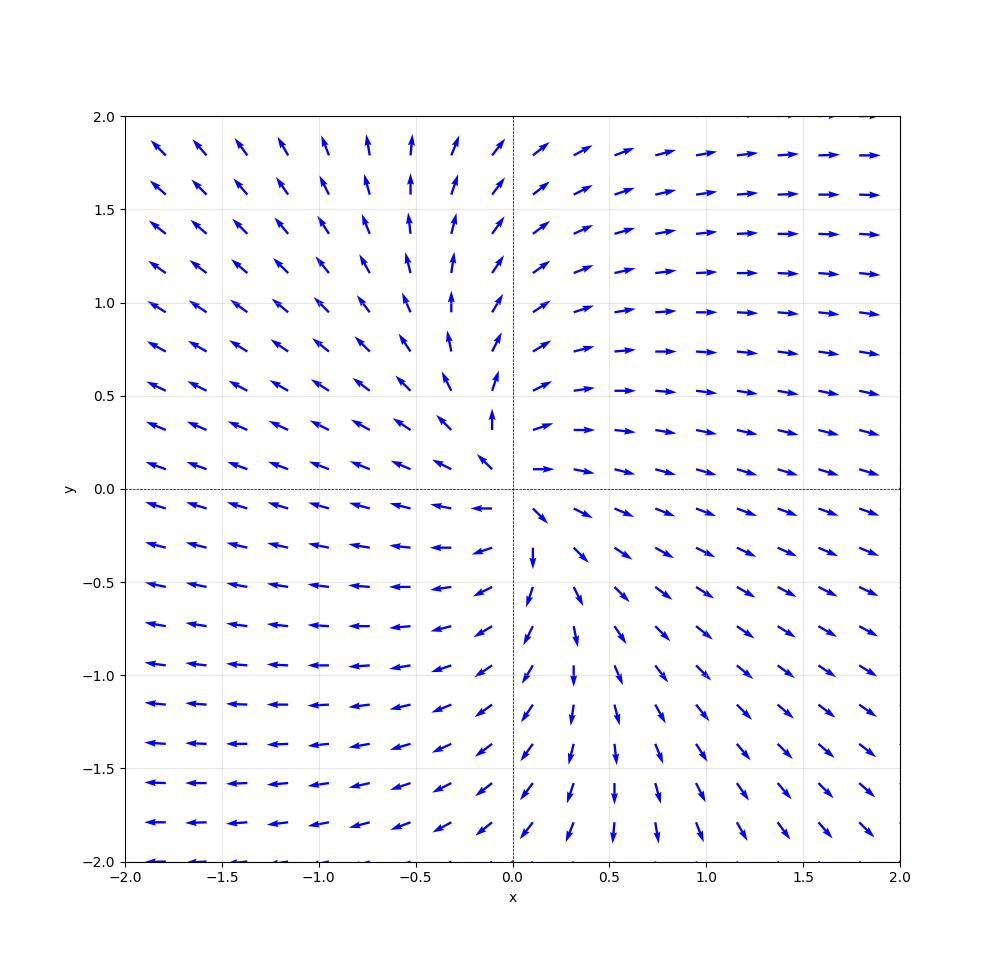
\includegraphics[width=0.8\linewidth]{graph/976.png}
                
        \label{fig:mpr}
        
    \end{figure}

\end{solution}\pagebreak

\section*{Задача 980}
Найти и исследовать особые точки.
$$
    y' = {2x + y}{x - 2y - 5}
$$

\begin{solution}
    $$\begin{cases}
            2x + y = 0 \\
            x - 2y - 5 = 0
        \end{cases} => x = 1, y = -2 $$
    Запишем матрицу 1-го приближения:
    $$ \tilde{A} = \begin{pmatrix}
            1 & -2 \\
            2 & 1
        \end{pmatrix} $$
    $$ |\tilde{A} - \lambda E| = \begin{vmatrix}
            1 - \lambda & -2          \\
            2           & 1 - \lambda
        \end{vmatrix} = (1 - \lambda)^2 + 4 = 0 $$
    $$ \lambda^2 - 2\lambda + 5 = 0 => $$
    $$ => \lambda_{1, 2} = 1 \pm 2 \cdot i => $$
    => фокус.
    \begin{figure}[h]
        \centering
        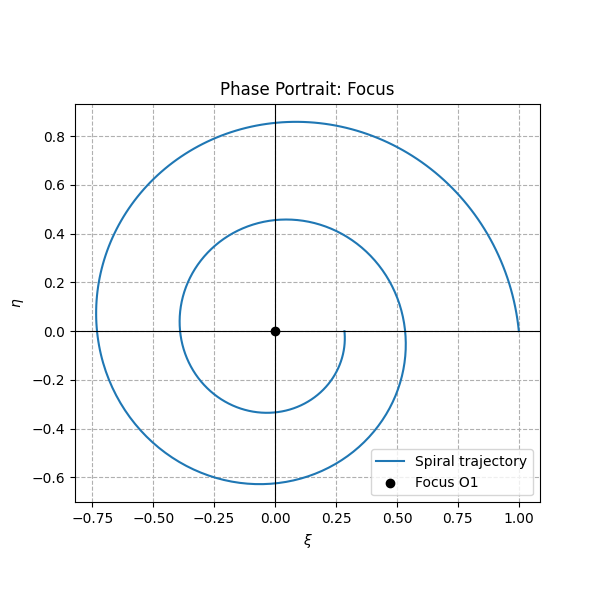
\includegraphics[width=0.8\linewidth]{graph/980.png}
    \end{figure}
\end{solution}
% \section*{Нелинейные системы}
1 способ. Метод исключения неизвестных. \par
2 способ. Решение путем отыскания интег интеграций. Пример:
$$ \dfrac{dx}{xz} = \dfrac{dy}{yz} = \dfrac{dz}{-xy} = dt $$
$$ \begin{cases}
        \dfrac{dx}{dt} = xz \\
        \dfrac{dy}{dt} = yz \\
        \dfrac{dz}{dt} = -xy
    \end{cases} $$

$$ \begin{cases}
        x = xy \\
        y = yz \\
        z = -xy
    \end{cases} $$

$$ \dfrac{dx}{xz} = \dfrac{dy}{yz} $$
$$ \ln{|x|} = \ln{|y|} + C $$
$$ x = Cy $$
$$ \dfrac{x}{y} = C $$
$$ \dfrac{dx}{xz} = \dfrac{dy}{yz} = \dfrac{dz}{-xy} = \dfrac{ydx + xdy}{xyz + xyz} $$
$$ -z^2 = xy - C _2 $$
$$
    \begin{cases}
        \dfrac{x}{y} = C_1 
        z^2 + xy = C_2 
    \end{cases}
$$

Обозначим левые части как $ \phi_1 и \phi_2 $ соответственно. Тогда:

$$
    \begin{vmatrix}
        \dfrac{\delta \phi_1}{\delta x} & \dfrac{\delta \phi_1}{\delta y} \\
        \dfrac{\delta \phi_2}{\delta x} & \dfrac{\delta \phi_2}{\delta y}
    \end{vmatrix} \not\equiv 0
$$

% \section*{Номер 1141}
% $$
%     \begin{cases}
%         y' = \dfrac{x}{z} \\
%         z' = -\dfrac{x}{y}
%     \end{cases}
% $$

% $$
%     \begin{cases}
%         x = y'z \\
%         x = -y z'
%     \end{cases}
% $$

$$ u' = F(t, u) $$
$$ \dfrac{\delta \phi}{\delta t} + \sum_{i} \dfrac{\delta \phi}{\delta u_i} F(t, u) = 0 $$
\section*{Номер 1161}
$$ \begin{cases}
    \dfrac{dx}{dt} = \dfrac{x^2 - t}{y} = F_1 \\
    \dfrac{dy}{dt} = -x = F_2
\end{cases} $$
$\phi_1 = t^2 + 2xy, \phi_2 = x^2 - ty$\par
$$ \dfrac{\delta \phi_1}{\delta t} = 2t  $$
$$ \dfrac{\delta \phi_1}{\delta x} = 2y $$
$$ \dfrac{\delta \phi_1}{\delta y} = 2x $$
Тогда: 
$$ 2t + 2y \cdot \dfrac{x^2 - t}{y} + 2x \cdot (-x) = 0 $$
$$ 0 = 0 $$

\section*{Номер 1145}
$$ \begin{cases}
        2zy' = y^2 - z^2 + 1 \\
        z' = z + y
    \end{cases} $$

\begin{solution}
    $$
        \begin{cases}
            2z(z' - z)' = (z' - z)^2 - z^2 + 1 \\
            y = z' - z
        \end{cases}
    $$
    $$ 2zz'' - 2zz' = (z')^2 - 2z'z + z^2 - z^2 + 1 $$
    $$ 2zz'' - (z')^2 - 1 = 0 \text{ - понизить порядок. } $$
    Нет явно заданного аргумента => замена $ z' = p(z); z'' = p_z'\cdot p $
    $$ 2z \cdot p'p - p^2 - 1 = 0 $$
    $$ 2z \cdot \dfrac{dp}{dz} \cdot p = p^2 + 1 = 0 | \cdot \dfrac{dz}{(p^2 + 1) \cdot 2z} $$
    $$ \int \dfrac{p}{p^2 + 1} dp = \int \dfrac{dz}{2z} = 0 $$
    Пусть $ t = p^2 + 1 $, $ t' = 2p $. Тогда: $ dp = \dfrac{1}{t'} dt => dp = \dfrac{1}{2p} dt $.
    $$ \int \dfrac{p}{p^2 + 1} dp = \int \dfrac{p}{2p \cdot t} dt = \dfrac{1}{2} \int \dfrac{dt}{t} = \dfrac{1}{2} \ln |t| $$
    $$ \dfrac{1}{2} \ln |p^2 + 1| = \dfrac{1}{2} \ln |z| - C $$
    $$ e^{\ln |p^2 + 1|} = e^{\ln |z| - C} $$
    $$ p^2 + 1 = \dfrac{z}{C_1} $$
    $$ p = \pm \sqrt{\dfrac{z}{C_1} - 1} $$
    $$ \dfrac{dz}{dx} = \pm \sqrt{\dfrac{z}{C_1} - 1} $$
    $$ \pm \int \dfrac{dz}{\sqrt{\dfrac{z}{C_1} - 1}} = \int dx $$
    $$ \pm 2 \sqrt{C_1 z - C_1^2} + C_2 = x + C_3 \text{ => } $$
    => $ z = C_1 + \dfrac{1}{4 C_1} (x + C_2)^2 $ => \par
    \textbf{Ответ: $ y = z' - z = \dfrac{1}{C_2} (x + C_2) - \dfrac{1}{4 C_1} (x + C_2)^2 - C_1 $}

\end{solution}\pagebreak
\section*{Номер 1153}

$$ \dfrac{dx}{z^2 - y^2} = \dfrac{dy}{z} = \dfrac{dz}{-y} $$

\begin{solution}
    $$ \dfrac{dx}{z^2 - y^2} = \dfrac{dy}{z} = \dfrac{dz}{-y} = \dfrac{zdy + ydz}{z^ - y^2} $$
    $$ \dfrac{dx}{z^2 - y^2} = \dfrac{zdy + ydz}{z^2 - y^2} $$
    $$ \int dx = \int d(zy) $$
    $$ x = zy + C_1 $$
    $$ C_1 = x - zy $$
    $$ \dfrac{dy}{z} = - \dfrac{dz}{y} \text{ => } \int zdz \text{ => } y^2 + z^2 = C_2 $$
    \textbf{Ответ: $ C_1 = x - zy, C_2 = y^2 + z^2 $}

\end{solution}\pagebreak
\section*{Номер 1163}
$$ \dfrac{dx}{y} = - \dfrac{dy}{x} = \dfrac{dz}{u} = - \dfrac{du}{z} $$

\begin{solution}
    Пусть $ \phi = yz - ux $. Тогда:
    $$ \dfrac{\delta \phi}{\delta y} = z; \dfrac{\delta \phi}{\delta z} = y; \dfrac{\delta \phi}{\delta u} = -x; \dfrac{\delta \phi}{\delta x} = -u $$
    Проверить, чтобы $ \dfrac{\delta \phi}{\delta x} \cdot F_x + \dfrac{\delta \phi}{\delta y} \cdot F_y + \dfrac{\delta \phi}{\delta z} \cdot F_z + \dfrac{\delta \phi}{\delta u} \cdot F_u = 0 $
    $$ \dfrac{dx}{y} = - \dfrac{dy}{x} => F_x = y; F_y = -x $$
    $$ \dfrac{dz}{u} = - \dfrac{du}{z} => F_u = -z; F_z = u $$
    Имеем: $ -u \cdot y + z \cdot (-x) + y \cdot u + (-x) \cdot (-z) = 0 $
    $$ 0 = 0 \text{ => $\phi$ - первый $\int$-л системы} $$


\end{solution}\pagebreak
\section*{Номер 1180}
$$ (z - y)^2 \dfrac{\delta z}{\delta x} + xz \cdot \dfrac{\delta z}{\delta y} = xy $$

\begin{solution}
    $$ \dfrac{dx}{(z - y)^2} = \dfrac{dy}{xz} = \dfrac{dz}{xy} $$
    \begin{itemize}
        \item
              $$ \dfrac{dy}{xz} = \dfrac{dz}{xy};\quad \dfrac{dy}{z} = \dfrac{dz}{y};\quad \int ydy = \int zdz $$
              $$ y^2 - z^2 = C_1 $$
        \item
              $$ \dfrac{dy - dz}{x(z - y)} = \dfrac{dx}{(z - y)^2};\quad \dfrac{dy - dz}{x} = \dfrac{dx}{z - y} $$
              $$ (z - y) \cdot d(z - y) + xdx = 0 $$
              $$ d((z - y)^2 + x^2) = 0\quad => \quad (z - y)^2 + x^2 = C_2 $$
    \end{itemize}
    $$ F(y^2 - z^2, x^2 + (z - y)^2) = 0 $$

\end{solution}

\section*{Номер 1182}
$$ y \dfrac{\delta z}{\delta x} + z \dfrac{\delta z}{\delta y} = \dfrac{y}{x} $$

\begin{solution}
    $$ \dfrac{dx}{y} = \dfrac{dy}{z} = x \dfrac{dz}{y} $$
    \begin{itemize}
        \item
              $$ \dfrac{dx}{y} = \dfrac{xdz}{y};\quad \int \dfrac{dx}{x} = \int dz \quad => \quad \ln |x| = z + C_1 $$
        \item
              $$ \dfrac{dx}{y} = \dfrac{dy}{z},\quad z = \ln |x| - C_1 $$
              $$ dx \cdot (\ln |x| - C_1) = ydy $$
              $$ \int \ln |x| dx - \int C_1 dx = \int ydy $$
              $$ \int \ln |x| \cdot 1 dx = \ln x \cdot x - \int x \cdot \dfrac{1}{x} dx = \ln x \cdot x - x $$
        \item
              $$ x \cdot ln|x| - x - x C_1 = \dfrac{1}{2} y^2 + C_2 $$
              $$ -x + xz - \dfrac{1}{2} y^2 = C_2 $$
              $$ -2x + 2xz - y^2 = C_2 $$
    \end{itemize}
    $$ F(\ln|x| - z, 2x(z - 1) - y^2) = 0 $$
\end{solution}\pagebreak
\section*{Номер 1198}

$$
    \begin{cases}
        x \cdot \dfrac{\delta z}{\delta x} - y \cdot \dfrac{\delta z}{\delta y} = z^2 \cdot (x - 3y) \\
        x = 1                                                                                        \\
        yz + 1 = 0
    \end{cases}
$$

\begin{solution}
    $$ \dfrac{dx}{x} = \dfrac{dy}{-y} = \dfrac{dz}{z^2 (x - 3y)} $$
    \begin{itemize}
        \item
              $$ \int \dfrac{dx}{x} = \int \dfrac{dy}{-y}; \quad e^{\ln|x| + ln|y|} = e^{\ln C_1} $$
              $$ xy = C_1 $$
        \item
              $$ \dfrac{dy}{-y} = \dfrac{dz}{z^2 (x - 3y)}; \quad (x - 3y) \cdot \dfrac{dy}{-y} = \dfrac{dz}{z^2} $$
              $$ \int (-\dfrac{C_1}{y^2} + 3) \cdot dy = \int \dfrac{dz}{z^2} $$
              $$ \dfrac{C_1}{y} + 3y = - \dfrac{1}{z} + C_2 $$
        \item
              $$
                  \begin{cases}
                      C_1 = yx \quad=>\quad y \\
                      C_2 = 1 + 2 C_1         \\
                      x = 1                   \\
                      y = - \dfrac{1}{z}
                  \end{cases}
              $$
    \end{itemize}
    Получается, что $ C_1 = xy $ и $ C_2 = 1 + 2C_1 = x + 3y + \dfrac{1}{z} = 1 + 2xy $. \par
    \textbf{Ответ: $ 2xy + 1 = x + 3y + \dfrac{1}{z} $}

\end{solution}


\section*{Номер 1181}
$$ xy \dfrac{\delta z}{\delta x} + (x - 2z) \cdot \dfrac{\delta z}{\delta y} = yz $$

\begin{solution}

    $$ \dfrac{dx}{xy} = \dfrac{dy}{x - 2z} = \dfrac{dz}{yz} $$

    \begin{itemize}

        \item
              $$ \dfrac{dx}{xy} = \dfrac{dz}{yz};\quad \int \dfrac{dx}{x} = \int \dfrac{dz}{z}; $$
              $$ \ln |z| - \ln |x| = C_1\quad=>\quad\dfrac{z}{x} = C_1 $$
        \item
              $$ \dfrac{dx - 2dz}{y(x - 2z)} = \dfrac{dy}{x - 2z};\quad \int dx - \int 2dz = \int ydy $$
              $$ x - 2z - \dfrac{y^2}{2} = C_2 $$
              $$ 2x - 4z - y^2 = C_2 $$
    \end{itemize}

    \textbf{Ответ: $ F(\dfrac{z}{x}, 2x - 4z - y^2) = 0 $}

\end{solution}

\section*{Номер 1183}

$$ \sin^2x \cdot \dfrac{\delta z}{\delta x} + \tg z \cdot \dfrac{\delta z}{\delta y} = \cos^2x $$

\begin{solution}
    $$ \dfrac{dx}{\sin^2x} = \dfrac{dy}{\cos^2z} = \dfrac{dz}{cos^2z} $$

    \begin{itemize}
        \item
              $$  \int \dfrac{dx}{\sin^x} = \dfrac{dz}{\cos^z} $$
              $$ -\ctg x = \tg z + C_1 $$
              $$ C_1 = \tg z + \ctg x $$
        \item
              $$ \dfrac{dy}{\tg z} = \dfrac{dz}{\cos^2z};\quad \int \dfrac{\tg z}{\cos^2d}dz $$
              $$ \int \dfrac{\tg z}{\cos^2z} dz = \int \dfrac{\sin z}{\cos^3z} dz = \int \dfrac{1}{\cos^3z} d(\cos z) = \dfrac{1}{2 \cdot cos^2z} + C_2 $$
              $$ y = \dfrac{1}{2 \cdot \cos^2z} + C_2 $$
    \end{itemize}
    \textbf{Ответ: $ F(\tg z + \ctg x,\quad y - \dfrac{1}{2 \cdot \cos^2z}) $}
    
\end{solution}\pagebreak
\section*{Номер 1201}

$$ z \cdot \dfrac{\delta z}{\delta x} - xy \cdot \dfrac{\delta z}{\delta y} = 2xz; \quad x + y = 2; \quad yz = 1 $$

\begin{solution}
    $$ \dfrac{dx}{z} = \dfrac{dy}{-xy} = \dfrac{dz}{2xz} $$

    \begin{itemize}
        \item
              $$ \dfrac{dy}{-xy} = \dfrac{dz}{2xz}\quad=>\quad -2\int \dfrac{dy}{y} = \int \dfrac{dz}{z}; $$
              $$ e^{\ln |z| + \ln |y|^2} = e^{C_1} $$
              $$ y^2 z = C_1 $$
        \item
              $$ \dfrac{dx}{z} = \dfrac{dz}{2xz} \quad=>\quad \int 2xdx = \int dz; \quad x^2 + C_2 = z $$
              С учетом заданных доп. условий:
              $$
                  \begin{cases}
                      C_1 = y^2 z = yz \cdot y = y                    \\
                      C_2 = x^2 - z = (2 - y)^2 - z = (2 - C_1)^2 - z \\
                      x + y = 2 \quad=>\quad x = 2 - y                \\
                      yz = 1                                          \\
                  \end{cases}
              $$
    \end{itemize}
    \textbf{Ответ: $ (2 - y^2 z)^2 = x^2 $}
\end{solution}\pagebreak
\section*{Номер 772}
Рассмотрим дифференциальное уравнение:
\begin{equation}
    y'' = f(x)
\end{equation}
с граничными условиями:
\begin{equation}
    y(0) = 0, \quad y(x) \to 0 \text{ при } x \to +\infty.
\end{equation}

\begin{solution}
    \begin{itemize}
        \item Общее решение уравнения:
              \begin{equation}
                  y'' = 0 \Rightarrow y(x) = Ax + B.
              \end{equation}
        \item Для области $0 \leq x \leq s$:
              \begin{equation}
                  G(x,s) = Ax + B.
              \end{equation}
              Условие $G(s,s) = 0$ даёт $B = 0$, следовательно:
              \begin{equation}
                  G(x,s) = A x.
              \end{equation}
        \item Для области $x > s$:
              \begin{equation}
                  G(x,s) = Cx + D.
              \end{equation}
              Так как $G(x,s) \to 0$ при $x \to +\infty$, необходимо $C = 0$, откуда:
              \begin{equation}
                  G(x,s) = D.
              \end{equation}
        \item Условие разрыва первой производной:
              \begin{equation}
                  G'(s+0, s) - G'(s-0, s) = 1.
              \end{equation}
              Подставляя $G'(x,s)$:
              \begin{equation}
                  0 - A = 1 \Rightarrow A = -1.
              \end{equation}
              Так как $A s = D$, получаем $D = -s$.
    \end{itemize}

    Таким образом, функция Грина:
    \begin{equation}
        G(x,s) =
        \begin{cases}
            -x, & 0 \leq x \leq s, \\
            -s, & x \geq s.
        \end{cases}
    \end{equation}
\end{solution}\pagebreak
\section*{Номер 765}

\begin{solution}
    $$ y'' + y = f(x) \quad y = C_1 \cos x + C_2 \sin x $$
    $$ G(x, s) = A(s) \cos x + B(s) \sin x \text{, где  $0 \leq x \leq s$} $$
    $$ G'(0,s) = 0 $$
    $$ A(s)\sin(0) + B(s)\cos(0) = 0 \Rightarrow B(s) = 0 $$
    $$ G(x,s) = A(s) \cos(x) $$

    при $ s \leq x \leq \pi $.

    $$ G(x,s) = C(s) \cos(x) + D(s) \sin(x) $$
    $$ G(\pi,s) = 0: \quad C(s) \cos(\pi) + D(s) \sin(\pi) = 0 $$
    $$ C(s) = 0 $$
    $$ G(x,s) = D(s) \sin(x) $$
    $$ A(s) \cos(x) = D(s) \sin(x) $$
    $$ G'(s+0,s) - G(s-0,s) = 1 $$

    \begin{itemize}
        \item
              $$ D(s) \cos(s) = -A(s) \sin(s) = 1 $$
              $$ D(s) \cos(s) + A(s) \sin(s) = 1 $$
        \item
              $$
                  \begin{cases}
                      A(s) \cos(s) - D(s) \sin(s) = 1 \\
                      D(s) \cos(s) + A(s) \sin(s) = 1
                  \end{cases}
              $$
              Преобразуем:
              $$ A(s) \cos(s) + D(s) \cos^2(s) + A(s) \sin^2(s) = \cos(s) $$
              $$ A(s) (\sin^2(s) + \cos^2(s)) = \cos(s) $$
              $$ A(s) = \cos(s) $$
        \item
              $$ A(s) \cos(s) = D(s) \sin(s) \Rightarrow A(s) = \sin(s) $$
              $$ D(s) = \cos(s) $$
    \end{itemize}

    \textbf{Ответ:}

    $$
        G(x,s) =
        \begin{cases}
            \sin(s) \cos(x), \quad 0 \leq x \leq s, \\
            \cos(s) \sin(x), \quad s < x \leq \pi.
        \end{cases}
    $$

\end{solution}\pagebreak
\section*{Номер 770}

$$ xy'' - y' = 0 $$
$$ y'(1) = 0, \quad y(2) = 0 $$

\begin{solution}
    Обозначим $ z = y' $, тогда уравнение принимает вид:
    $$ xz' - z = 0 $$
    Решаем уравнение:

    $$ xz' = z $$
    $$ \dfrac{dz}{z} = \dfrac{dx}{x} $$
    $$ \ln |z| = \ln |x| + C $$

    $$ z = Cx $$

    $$ y' = Cx $$
    $$ y = \dfrac{Cx^2}{2} + C_1 $$
    Рассмотрим области $ 1 \leq x \leq s $:
    $$ G(x,s) = A(s) \dfrac{x^2}{2} + B(s) $$
    $$ G'(x,s) = A(s) x $$
    Так как $ G'(1,s) = 0 $, то:
    $$ A(s) = 0 $$
    $$ G(x,s) = B(s) $$
    Рассмотрим область $ s \leq x \leq 2 $:
    $$ G(x,s) = C(s) \dfrac{x^2}{2} + D(s) $$
    $$ C(s) \dfrac{2^2}{2} + D(s) = 0 $$
    $$ D(s) = -2C(s) $$
    $$ G(x,s) = C(s) \left( \dfrac{x^2}{2} - 2 \right) $$
    $$ G(s+0, s) - G(s-0, s) = 1 $$
    $$ C(s) s - 0 = 1 $$
    $$ C(s) = \dfrac{1}{s} $$

\end{solution}\pagebreak



\end{document}
